% flashcards-title: Model, prediction, and evidence comparison
% flashcards-desc: A simplified model leads to a conditional prediction. Observation or measurement provides evidence. Prediction and evidence both enter a comparison.
\documentclass[border=6pt]{standalone}
\def\pgfsysdriver{pgfsys-dvisvgm.def}
\usepackage{tikz}
\usetikzlibrary{arrows.meta,positioning,shapes.geometric}
\definecolor{mechInk}{HTML}{172033}
\definecolor{mechBlue}{HTML}{155EEF}
\definecolor{mechOrange}{HTML}{B54708}
\definecolor{mechPale}{HTML}{E8F0FF}
\definecolor{mechGray}{HTML}{667085}
\definecolor{mechLight}{HTML}{D0D5DD}
\tikzset{
  every picture/.style={font=\sffamily\large, text=mechInk},
  mech box/.style={draw=mechInk, line width=1.2pt, rounded corners=4pt,
    fill=white, align=center, minimum height=14mm, inner xsep=5mm},
  mech primary/.style={draw=mechBlue, line width=2.2pt},
  mech secondary/.style={draw=mechOrange, line width=2.2pt, dashed},
  mech guide/.style={draw=mechGray, line width=0.9pt, dashed},
  mech arrow/.style={-{Stealth[length=3.2mm,width=2.4mm]},
    draw=mechInk, line width=1.4pt, line cap=butt},
  mech axis/.style={draw=mechInk, line width=1.2pt},
  mech tick/.style={draw=mechInk, line width=1pt}
}

\begin{document}
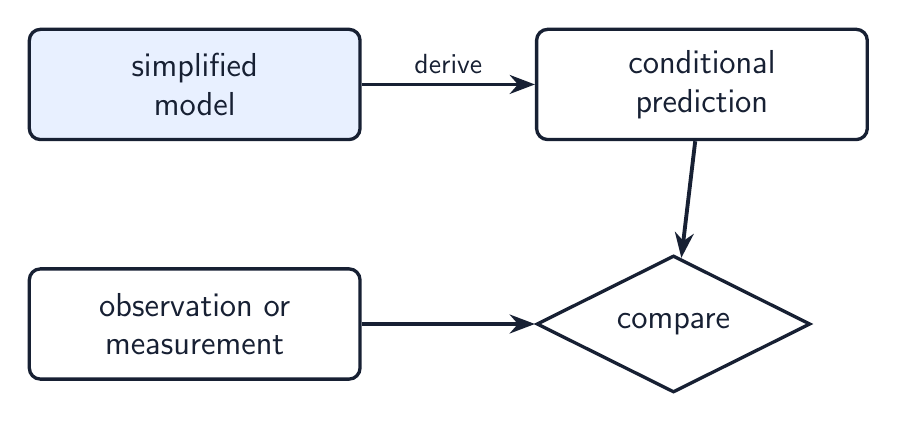
\begin{tikzpicture}[node distance=16mm and 22mm]
  \node[mech box, fill=mechPale, minimum width=42mm] (model) {simplified\\model};
  \node[mech box, right=of model, minimum width=42mm] (prediction) {conditional\\prediction};
  \node[mech box, below=of model, minimum width=42mm] (evidence) {observation or\\measurement};
  \node[diamond, draw=mechInk, line width=1.2pt, aspect=2,
    align=center, right=of evidence, fill=white, inner sep=2.5mm] (compare) {compare};
  \draw[mech arrow] (model) -- node[above, font=\sffamily\normalsize] {derive} (prediction);
  \draw[mech arrow] (prediction) -- (compare);
  \draw[mech arrow] (evidence) -- (compare);
\end{tikzpicture}
\end{document}
